%% ------------------------------------------------------------------------- %%n
\chapter{Descrição do Problema e Proposta}
\label{cap:Proposta}

O problema que estamos tratando, classificação de imagens de plâncton, enquadra-se na situação de dados não rotulados abundantes e com elevado custo de rotulação. Dado essa situação, o objetivo deste trabalho é o desenvolvimento de métodos para a rotulação e classificação rápida dessas imagens, a fim de que estudos posteriores, dependentes da classificação, tornem-se viáveis. 

Como foi visto no capítulo anterior, o aprendizado ativo poderia ser uma abordagem a ser utilizada para rotular um grande conjunto de amostras, com a ajuda de um especialista. Neste processo, o objetivo é a minimização do esforço de interação do usuário. Em seguida, uma vez em posse de amostras rotuladas, um classificafor pode ser treinado e utilizado para automaticamente classificar o restante das amostras não rotuladas.

Também conforme comentado no capítulo anterior, pesquisas recentes relacionadas à interação de usuários na tarefa de rotulação indicam as limitações do aprendizado ativo clássico. Nesse, o especialista tem uma atuação limitada de apenas confirmar ou corrigir o rótulo atribuído pelo algoritmo a algumas das amostras. Uma forma para contornar essas limitações são abordagens que colocam o especialista em um papel mais central, no qual= sua atuação passa a incluir a possibilidade de não só corrigir ou rotular amostras selecionadas pelo algoritmo, mas também participar no processo de seleção das amostras a serem rotuladas.

A proposta consiste em definirmos formas de interação do usuário, definir formas de usar a informação proveniente dessas interações, e avaliar a efetividade desse uso. Essas etapas estão descritas a seguir. Ao final descrevemos também o conjunto de dados e os procedimentos práticos que serão utilizados na parte experimental do trabalho.


\section{Estratégia de Interação}
\label{sec:estategia_interacao}

Duas ideias de interação ativa por parte de usuários estão  sendo consideradas nesta proposta. Como elas ainda não estão suficientemente amadurecidas, é possível que a estratégia final seja uma combinação delas.

\subsection{Interação Sobre o Espaço de Projeções}
\label{sec:espaco_projecoes}

Na classificação de imagens, tipicamente são extraídas um conjunto de características das imagens e elas são utilizadas pelos classificadores. No caso de plâncton, características explicitamente extraídas em geral estão relacionados à forma e textura dos organismos. Mais recentemente, com a popularização de redes neurais profundas e, especificamente, das redes convolucionais no caso de imagens, redes pré-treinadas em outros domínios de aplicação podem ser utilizadas como extratores de características. Isto é, dada uma rede pré-treinada, passa-se uma imagem para a rede e extrai-se os valores dessa rede em alguma camada de ativação. O conjunto de valores dessa camada é utilizada como uma representação da imagem de entrada.

Sejam características extraídas explicitamente ou implicitamente, elas podem ser representadas por um vetor em $\mathbb{R}^n$. A visualização de pontos em espaços de dimensão alta não é possível. Portanto, uma técnica comumente utilizada são as projeções desses pontos sobre o espaço 2D.

Existem diversos algoritmos que realizam essas projeções, também conhecidas por algoritmos de redução de dimensionalidade.= Várias delas são desenhadas para preservar certas propriedades dos dados no espaço original. Por exemplo, ...

(o t-SNE por exemplo, se não me engano, preserva a vizinhança; ou seja, os pontos mais próximos no espaço original aparecem como os mais próximos na projeção, embora a distância relativa não seja preservada).

As interações neste caso consistiriam de diferentes formas= do usuário interagir com os pontos no espaço 2D. Deve-se lembrar que cada ponto corresponde a uma imagem. Assim, durante a interação o usuário teria a possibildiade de explorar a estrutura de organização do conjunto de pontos e as imagens associadas a subconjuntos de pontos. Por exemplo, supondo que existam agrupamentos bem definidos na projeção, o usuário poderia inspecionar imagens de um desses agrupamentos e rapidamente determinar a classe predominante no grupo, excluindo apenas as que são de classes distintas.

À medida que mais e mais imagens são rotuladas, esses mapas de projeção viriam também acompanhados de cores associados aos pontos já rotulados. Isto poderia ser explorado pelo usuário para rotular amostras em regiões mais críticas (presença de amostras de classes distintass).




\subsection{Interação Sobre Galeria de Imagens} 
\label{sec:galeria_imagens}

Para rotular uma imagem, o especialista precisa ver o organismo presente na imagem. Dado que estamos pressupondo uma representação  das imagens como pontos no $R^
n$, podemos usar métricas de similaridade para selecionar grupos de imagens similares segundo essa métrica e exibir múltiplas imagens de um grupo simultaneamente.
 
Nesta situação, supondo-se que a maior parte dos organismos são de uma mesma classe, em poucas interações o especialista pode corrigir os rótulos errados e confirmar os demais como rótulos corretos.


\section{Uso das Informações Provenientes da Interação}
\label{sec:uso_das_informacoes_interacao}

A ideia básica do aprendizado ativo de iterar ciclos continua presente. A diferença básica é que o especialista poderá participar de forma mais ativa e selecionar as amostras a serem rotuladas.

A partir da definição de como ocorrerá essa interação, será possível também definir quais tipos de informação estarão disponíveis para o algoritmo gerar um novo classificador melhorado.



\section{Avaliação do Método}
\label{sec:avaliação do método}

texto texto texto texto texto texto texto texto texto texto texto texto texto texto texto texto texto texto texto texto texto texto texto texto texto texto texto texto texto texto texto texto texto texto texto texto texto texto texto texto texto texto texto texto texto 

\section{Considerações sobre a parte experimental}
\label{sec:consideracoes_parte_experimental}


\subsection{Base de Dados que Poderão ser Usados} 
\label{sec:base_usadas}

Neste trabalho teremos três bases de dados disponíveis. As especificações de cada uma estão a seguir.

\textbf{LAPS}

Este dataset foi desenvolvido pelo LAPS\footnote{LAPS: Laboratório de Sistemas Planctônicos (LAPS) do Departamento de Oceanografia Biológica, pertencente ao Instituto Oceanográfico da Universidade de São Paulo (IOUSP)} e contém 5.198 imagens de zooplanctons, divididas em 20 classes.

\textbf{NDSB}

Temos cerca de 30.000 imagens de zooplanctons, divididas em 121 classes, coletadas pelo Centro de Ciências Marinhas Hatfield da Universidade Estadual do Oregon. A fitura ~\ref{fig:ndsb} mostra alguns exemplos das imagens.

\begin{figure}
  \centering
  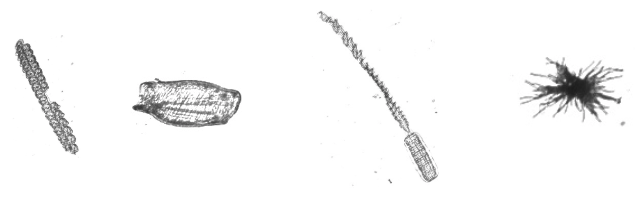
\includegraphics[width=1.0\textwidth]{figures/ndsb_exemplos.png}
  \caption{Exemplos de amostras do dataset NDSB}
  \label{fig:ndsb}
\end{figure}

\textbf{Japan}
Neste dataset temos 32.835 imagens divididas em 23 classes. A figura ~\ref{fig:japan} mostra alguns exemplos das imagens.


\begin{figure}
  \centering
  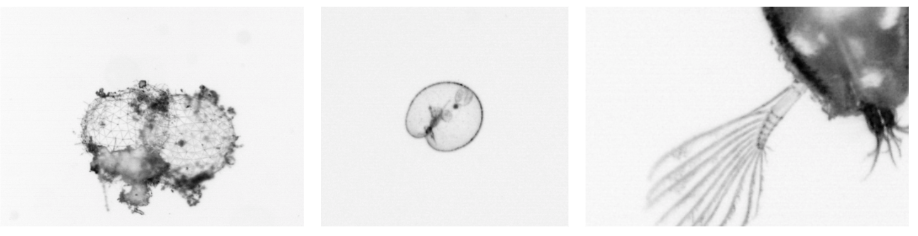
\includegraphics[width=1.1\textwidth]{figures/japan_exemplos.png}
  \caption{Exemplos de amostras do dataset Japan}
  \label{fig:japan}
\end{figure}




\subsection{Procedimento Prático} 
\label{sec:procedimento_pratico}

As amostras no datasets acima listados são rotulados. Desta forma, no caso do aprendizado ativo podemos facilmente simular o oráculo. texto texto texto texto texto texto texto texto texto texto texto texto texto texto texto texto texto texto texto texto texto texto texto texto texto texto texto texto texto texto texto texto texto texto texto texto texto texto texto texto texto texto texto texto texto texto texto texto texto texto texto texto texto texto texto texto texto texto texto texto texto texto texto texto texto texto texto texto texto          



%%%%%%%%%%%%%%%%%%%%%%%%%%%%%%%%%%%%%%%%%%%%%%%%%%%%%%%%%%%%%%%%%%
\section{Aprendizado Ativo Integrado com o Conhecimento Humano Especializado}
\label{sec:aprendizado_ativo_conhecimento_humano}

O Aprendizado Ativo é uma abordagem interessante quando precisamos diminuir o esforço de rotulação e ainda gerarmos um classificador decente. Como visto no capítulo anterior, estudos recentes tentam incorporar o conhecimento humano nesse framework [\cite{castro2009human, kottke2018other}], sendo que uma maneira interessante de se fazer isso é através da interação do humano com a visualização de dados [\cite{yang2018visually, bernard2018comparing, weigl2016mapview}]. Além disso, no caso dos plânctons, estudos mostram que a incorporação de conhecimentos de especialistas aumenta a acurácia dos modelos [\cite{benfield2007rapid}].

A figura ~\ref{fig:frameworks_AL} à esquerda mostra o framework clássico do Aprendizado Ativo. Nele temos cinco passos, sendo: i) um conjunto de dados não rotulados. No inicio do ciclo de aprendizado ativo teremos apenas alguns exemplos com rótulo correto para que já exista uma primeira versão de um classificador, ii) através de uma função matemática o algoritmo selecionará as amostras que tem menos certeza das categorias, iii) o classificador categoriza as amostras, iv) o oráculo valida ou corrige e v) o classificador incorpora as amostras corretas para o treinamento. Após isso as fases se repetem até algum critério de parada.

\begin{figure}
  \centering
  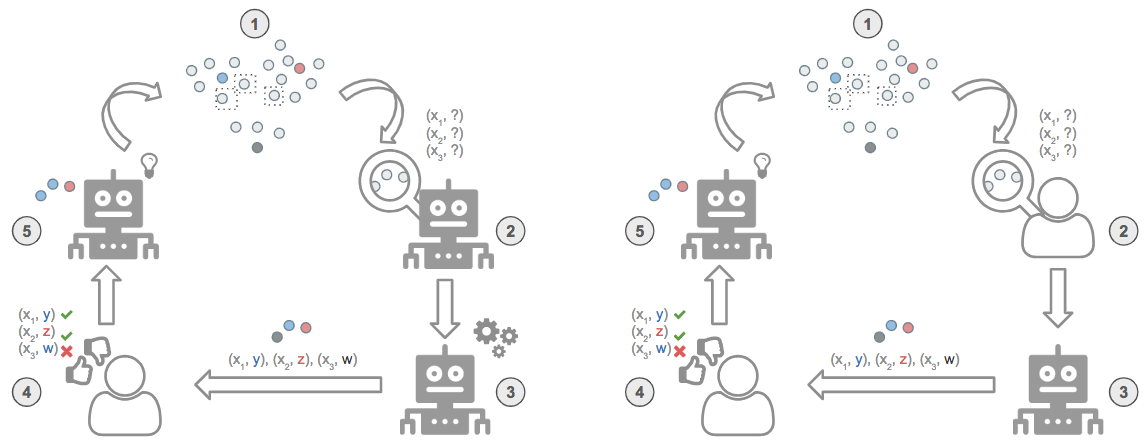
\includegraphics[width=0.95\textwidth]{figures/Frameworks_Active_Learning.png}
  \caption{esq: Framework Aprendizado Ativo Clássico, dir: Framework Aprendizado Ativo com Interação Humana na Seleção de Amostras}
  \label{fig:frameworks_AL}
\end{figure}

No caso do ciclo clássico, o oráculo serve apenas para validar as amostras do classificador. Como citado no capítulo fundamental teórico, essa atuação acaba fazendo com limitemos muito a atuação do especialista. Nossa proposta é fazer com que o oráculo seja, além de um validador, um selecionador de amostras [\cite{kottke2018other}]. A mesma figura à direita ilustra essa situação. A diferença é que no passo dois o oráculo também é responsável por selecionar os exemplos que considera mais representativo. 

A maneira pela qual será possível escolher os exemplos será através da projeção do espaço de features em um plano 2D, já que, geralmente, esse espaço possui uma alta dimensionalidade. O que queremos é encontrar uma transformação tal que $\mathcal{R}^d \xrightarrow{} \mathcal{R}^c$, com $c \ll d$ [\cite{van2009dimensionality}]. Será através dessa projeção que o especialista poderá selecionar os dados que ele acredita serem os mais representativos no ciclo para incorporar no ciclo de aprendizado ativo. 

%\section{Extração de Features}
%\label{sec:extracao_features}

%A extração de features será feita através de uma arquitetura de Deep Learning. 


%\section{Projeção do Espaço de Features}
%\label{sec:projecao_espaco_features}
